\section{Exploring Cubes with TikZ}

Cubes are one of the most fundamental shapes in both geometry and everyday life. Characterized by their six square faces, eight vertices, and twelve edges, cubes are a prime example of a three-dimensional square. They can be found in various contexts, from architecture and design to natural formations. In mathematics, cubes are studied not only for their geometric properties but also for their applications in algebra, where the cube of a number is its third power.

\begin{figure}[ht]
\centering % Centers the figure
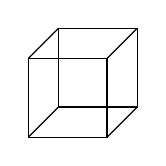
\begin{tikzpicture}
    % Bottom face
    \draw (0,0,0) -- (1,0,0) -- (1,1,0) -- (0,1,0) -- cycle;
    % Top face
    \draw (0,0,1) -- (1,0,1) -- (1,1,1) -- (0,1,1) -- cycle;
    % Side edges
    \draw (0,0,0) -- (0,0,1);
    \draw (1,0,0) -- (1,0,1);
    \draw (1,1,0) -- (1,1,1);
    \draw (0,1,0) -- (0,1,1);
\end{tikzpicture}
\caption{A simple 3D cube drawn with TikZ.} % Adds your caption here
\label{fig:3dcube} % Labels the figure for cross-referencing
\end{figure}

The cube illustrated above is created using TikZ, a powerful tool for generating vector graphics directly in LaTeX documents. Through simple commands, TikZ allows for precise control over the drawing, enabling the creation of both simple diagrams like this cube and more complex figures. The cube's representation here, while simple, serves as a foundational example for more intricate geometric constructions and visualizations in LaTeX. Learning to draw with TikZ not only enhances your documents visually but also provides a deeper understanding of the geometric concepts being presented.
